\documentclass[xcolor={usenames, table, x11names}, final, 10pt]{beamer}
\usetheme[
%%% option passed to the outer theme
% progressstyle=fixedCircCnt,   % fixedCircCnt, movingCircCnt (moving is deault)
]{Feather}

% If you want to change the colors of the various elements in the theme, edit and uncomment the following lines

% Change the bar colors:
% \setbeamercolor{Feather}{fg=red!20,bg=red}

% Change the color of the structural elements:
% \setbeamercolor{structure}{fg=red}

% Change the frame title text color:
% \setbeamercolor{frametitle}{fg=blue}

% Change the normal text color background:
% \setbeamercolor{normal text}{fg=black,bg=gray!10}

% -------------------------------------------------------
% INCLUDE PACKAGES
% -------------------------------------------------------

\usepackage[utf8]{inputenc}
\usepackage[italian]{babel}
\usepackage[T1]{fontenc}
\usepackage{helvet}
\usepackage{pgfplots}
\usepackage{ragged2e}
\usepackage{ocg-p}
\usepackage{blindtext}
\usepackage{hyperref}
\usepackage{pgfplots, pgfplotstable}
\usepackage{siunitx}
\usepackage{placeins}
\usepackage{datetime}
\usepackage{animate}
\usepackage{tikz}
\usepackage{graphics}
\usepackage[table]{xcolor} % richiesto per colortbl
% \usepackage{tabu} %per colorare il testo delle tabelle, non lo sfondo lez 11
\usepackage{booktabs}
\newdate{date}{21}{12}{2017}

% -------------------------------------------------------
% DEFINING AND REDEFINING COMMANDS
% -------------------------------------------------------

% colored hyperlinks
\newcommand{\chref}[2]{
  \href{#1}{{\usebeamercolor[bg]{Feather}#2}}
}

% -------------------------------------------------------
% INFORMATION IN THE TITLE PAGE
% -------------------------------------------------------
% \setbeamertemplate{title page}
% {
\title[25 anni di conduzione biologica in area Mediterranea: uno
studio di fisica del suolo] % [] is optional - is placed on the bottom of the
% sidebar on every slide
{ Caratteristiche fisico-strutturali di suoli in area Mediterranea
  sottoposti a diversi metodi di conduzione e lavorazione}


% \subtitle[Uno studio di fisica del suolo]{
% Uno studio di fisica del suolo
% }

\author[Simone Massenzio]{ 
  Candidato: Simone Massenzio \\
  Relatore: Dott. O.L. Pantani\\
  \vspace{0.1cm}
  Correlatori:
  Dott. L.P. D'Acqui, Prof. G.C. Pacini}     



\institute[] { \emph{Dipartimento di Scienze della Produzioni Animali e
    dell'Ambiente\\
    Universit\`a degli Studi di Firenze - UniFI\\}
  
  % there must be an empty line above this line - otherwise some
  % unwanted space is added between the university and the country (I
  %   % do not know why;( )
}

\date{\displaydate{date}}


% -------------------------------------------------------
% THE BODY OF THE PRESENTATION
% -------------------------------------------------------
\setbeamercovered{transparent}


\begin{document}
{\1
  \begin{frame}[noframenumbering]%{\footnotesize{Dipartimento di Scienze della Produzioni Animali e
    % dell'Ambiente\\
    % Universit\`a degli studi di Firenze - UniFI}}
    \titlepage
  \end{frame}}


% presumo che queste righe mettano dei segnali in ogni parte e sezione
% \AtBeginPart{\frame<beamer>{\partpage
% \transsplitverticalout[duration=1] 
% \begin{block}{}
%       %   \tableofcontents[subsectionstyle=show]
%   \tableofcontents[subsectionstyle=hide]
% \end{block}
% }}

%   \AtBeginSection[]{\frame<beamer>{%
%   \begin{block}{}
%     \tableofcontents[currentsection, subsectionstyle=hide]
%   \end{block}
% }
% }

\begin{frame}
  \vspace{2cm}
  
  \centering
  \includegraphics[width=0.8\textwidth]{../foto/wordcloud.png}
  
\end{frame}

\begin{frame}{Parte 1 \small{Montepaldi Long Term Experiment (MoLTE)}}
  \begin{columns}
    \column[T]{.42\textwidth}
    
    \begin{itemize}[<+->]
      \item MoLTE, esperimento a lungo termine di comparazione tra
        agricoltura biologica e convenzionale più duraturo di tutta
        l'area mediterranea
      \item \emph{Progetto Fertilcrop} Progetto del programma Horizon
        2020
     \emph{Sviluppare tecniche di gestione sostenibili ed efficienti per
    incrementare la produttività nei sistemi agricoli biologici}
    \end{itemize}

    \column[T]{.55\textwidth}
    \only<2>{
      \vspace{1cm}
      \begin{figure}
    \centering
    \includegraphics[width=0.6\textwidth]{../foto/FertilCropLogo.png}
    \end{figure}}
  \end{columns}
\end{frame}

\begin{frame}{Parte 1 \small{Fertilità del suolo e agricoltura biologica}}
  \begin{columns}
    \column{.32\textwidth} 
    Agricoltura biologica:
    \begin{itemize}[<+->]
      \pause
    \item suscita interesse commerciale
    \item non utilizza prodotti di sintesi
    \item mira a chiudere il ciclo dei nutrienti e dell'energia dell'agroecosistema
    \item pone maggiore attenzione alla fertilità del suolo
    \end{itemize}
    \
    \column{.65\textwidth}
    \only<3>{
      % \vspace{1.5cm}
      
      \centering
      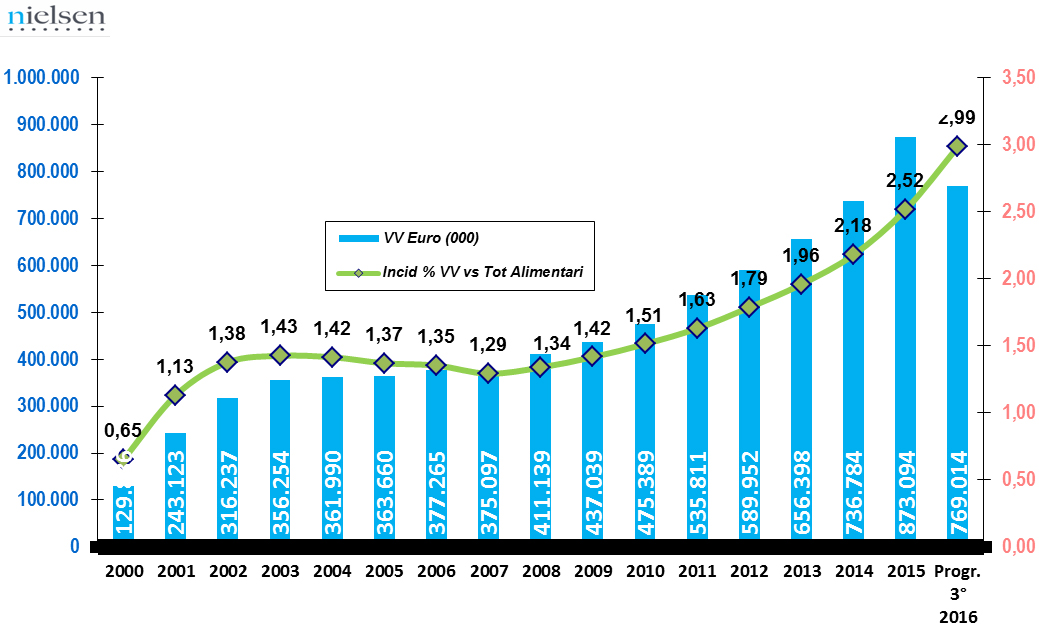
\includegraphics[width=\textwidth]{../foto/crescitaBio.jpg}
    }
    \only<2>{
      % \vspace{1.5cm}
      
      \centering
      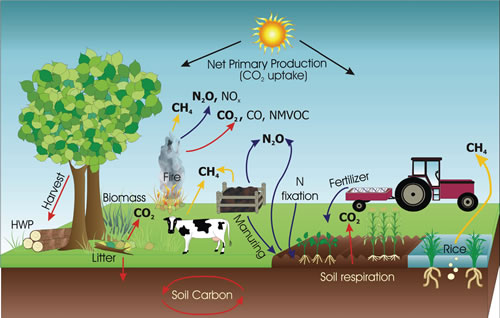
\includegraphics[width=\textwidth]{../foto/carbonCycle.jpg}
    }
    \only<4>{
      % \vspace{1.5cm}
      
      \centering
      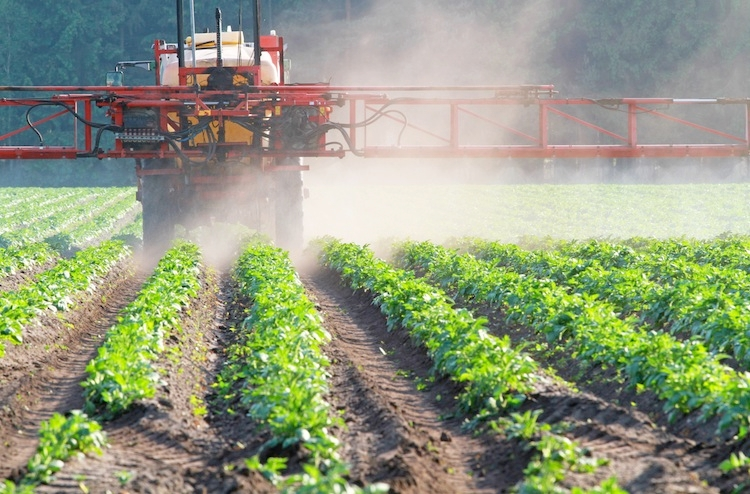
\includegraphics[width=\textwidth]{../foto/fitofarmaci.jpg}
    }
    \only<5>{
      % \vspace{1.5cm}
      
      \centering
      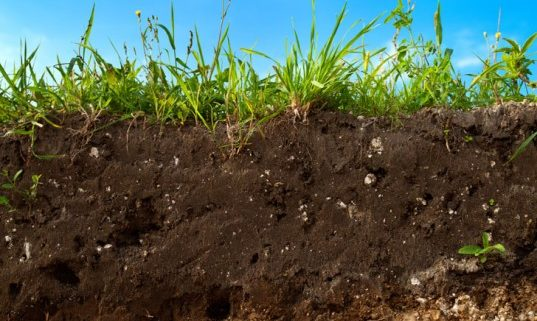
\includegraphics[width=\textwidth]{../foto/fertilitsuolo.jpg}
    }
  \end{columns}
\end{frame}



\begin{frame}{Parte 1 \small{Valutazione della fertilità}}
  Per valutare l'effetto dell'agricoltura biologica sulla fertilità
  vengono comunemente utilizzati parametri:
  \begin{itemize}[<+->]
    \pause
  \item Chimici
  \item Biologici
  \item Ecologici
  \item Produttivi
  \item \temporal<7>{Fisici}{\LARGE Fisici}{\LARGE Fisici}
    % \onslide<7->{\Large{$\rightarrow$ trascurati dalla letteratura}}

    \begin{enumerate}[<+->]
      \pause
    \item  \large{Densità apparente},\\ \normalsize{rapporto tra fase
        solida e spazi vuoti}
      \vfill
    \item \large{Stabilità di struttura degli aggregati},\\
      \normalsize{studio della dinamica della fase solida} 
      \vfill
    \item  \large{Distribuzione della dimensione dei pori},\\ \normalsize{studio degli spazi vuoti}
    \end{enumerate}
  \end{itemize}
  
\end{frame}



\begin{frame}{Parte 1 \small{Obiettivi}}
  Tramite l'uso di parametri di fertilità del suolo, verificare la
  presenza di eventuali differenze tra:
  \begin{columns}[c]
    \column{.50\textwidth}
    \begin{itemize}
    \item<2-> Metodo di conduzione
      \begin{itemize}
      \item <2->      convenzionale
      \item <2->      biologico
      \end{itemize}
    \item<3-> Lavorazioni primarie
      \begin{itemize}
      \item <3->      aratura, 
      \item <3->      frangizollatura
      \item <3->      rippatura        
      \end{itemize}
    \end{itemize}
    \column{.48\textwidth}
    \temporal<2>{}{\includegraphics[width=0.8\textwidth]{../foto/logo-Bio.png}}{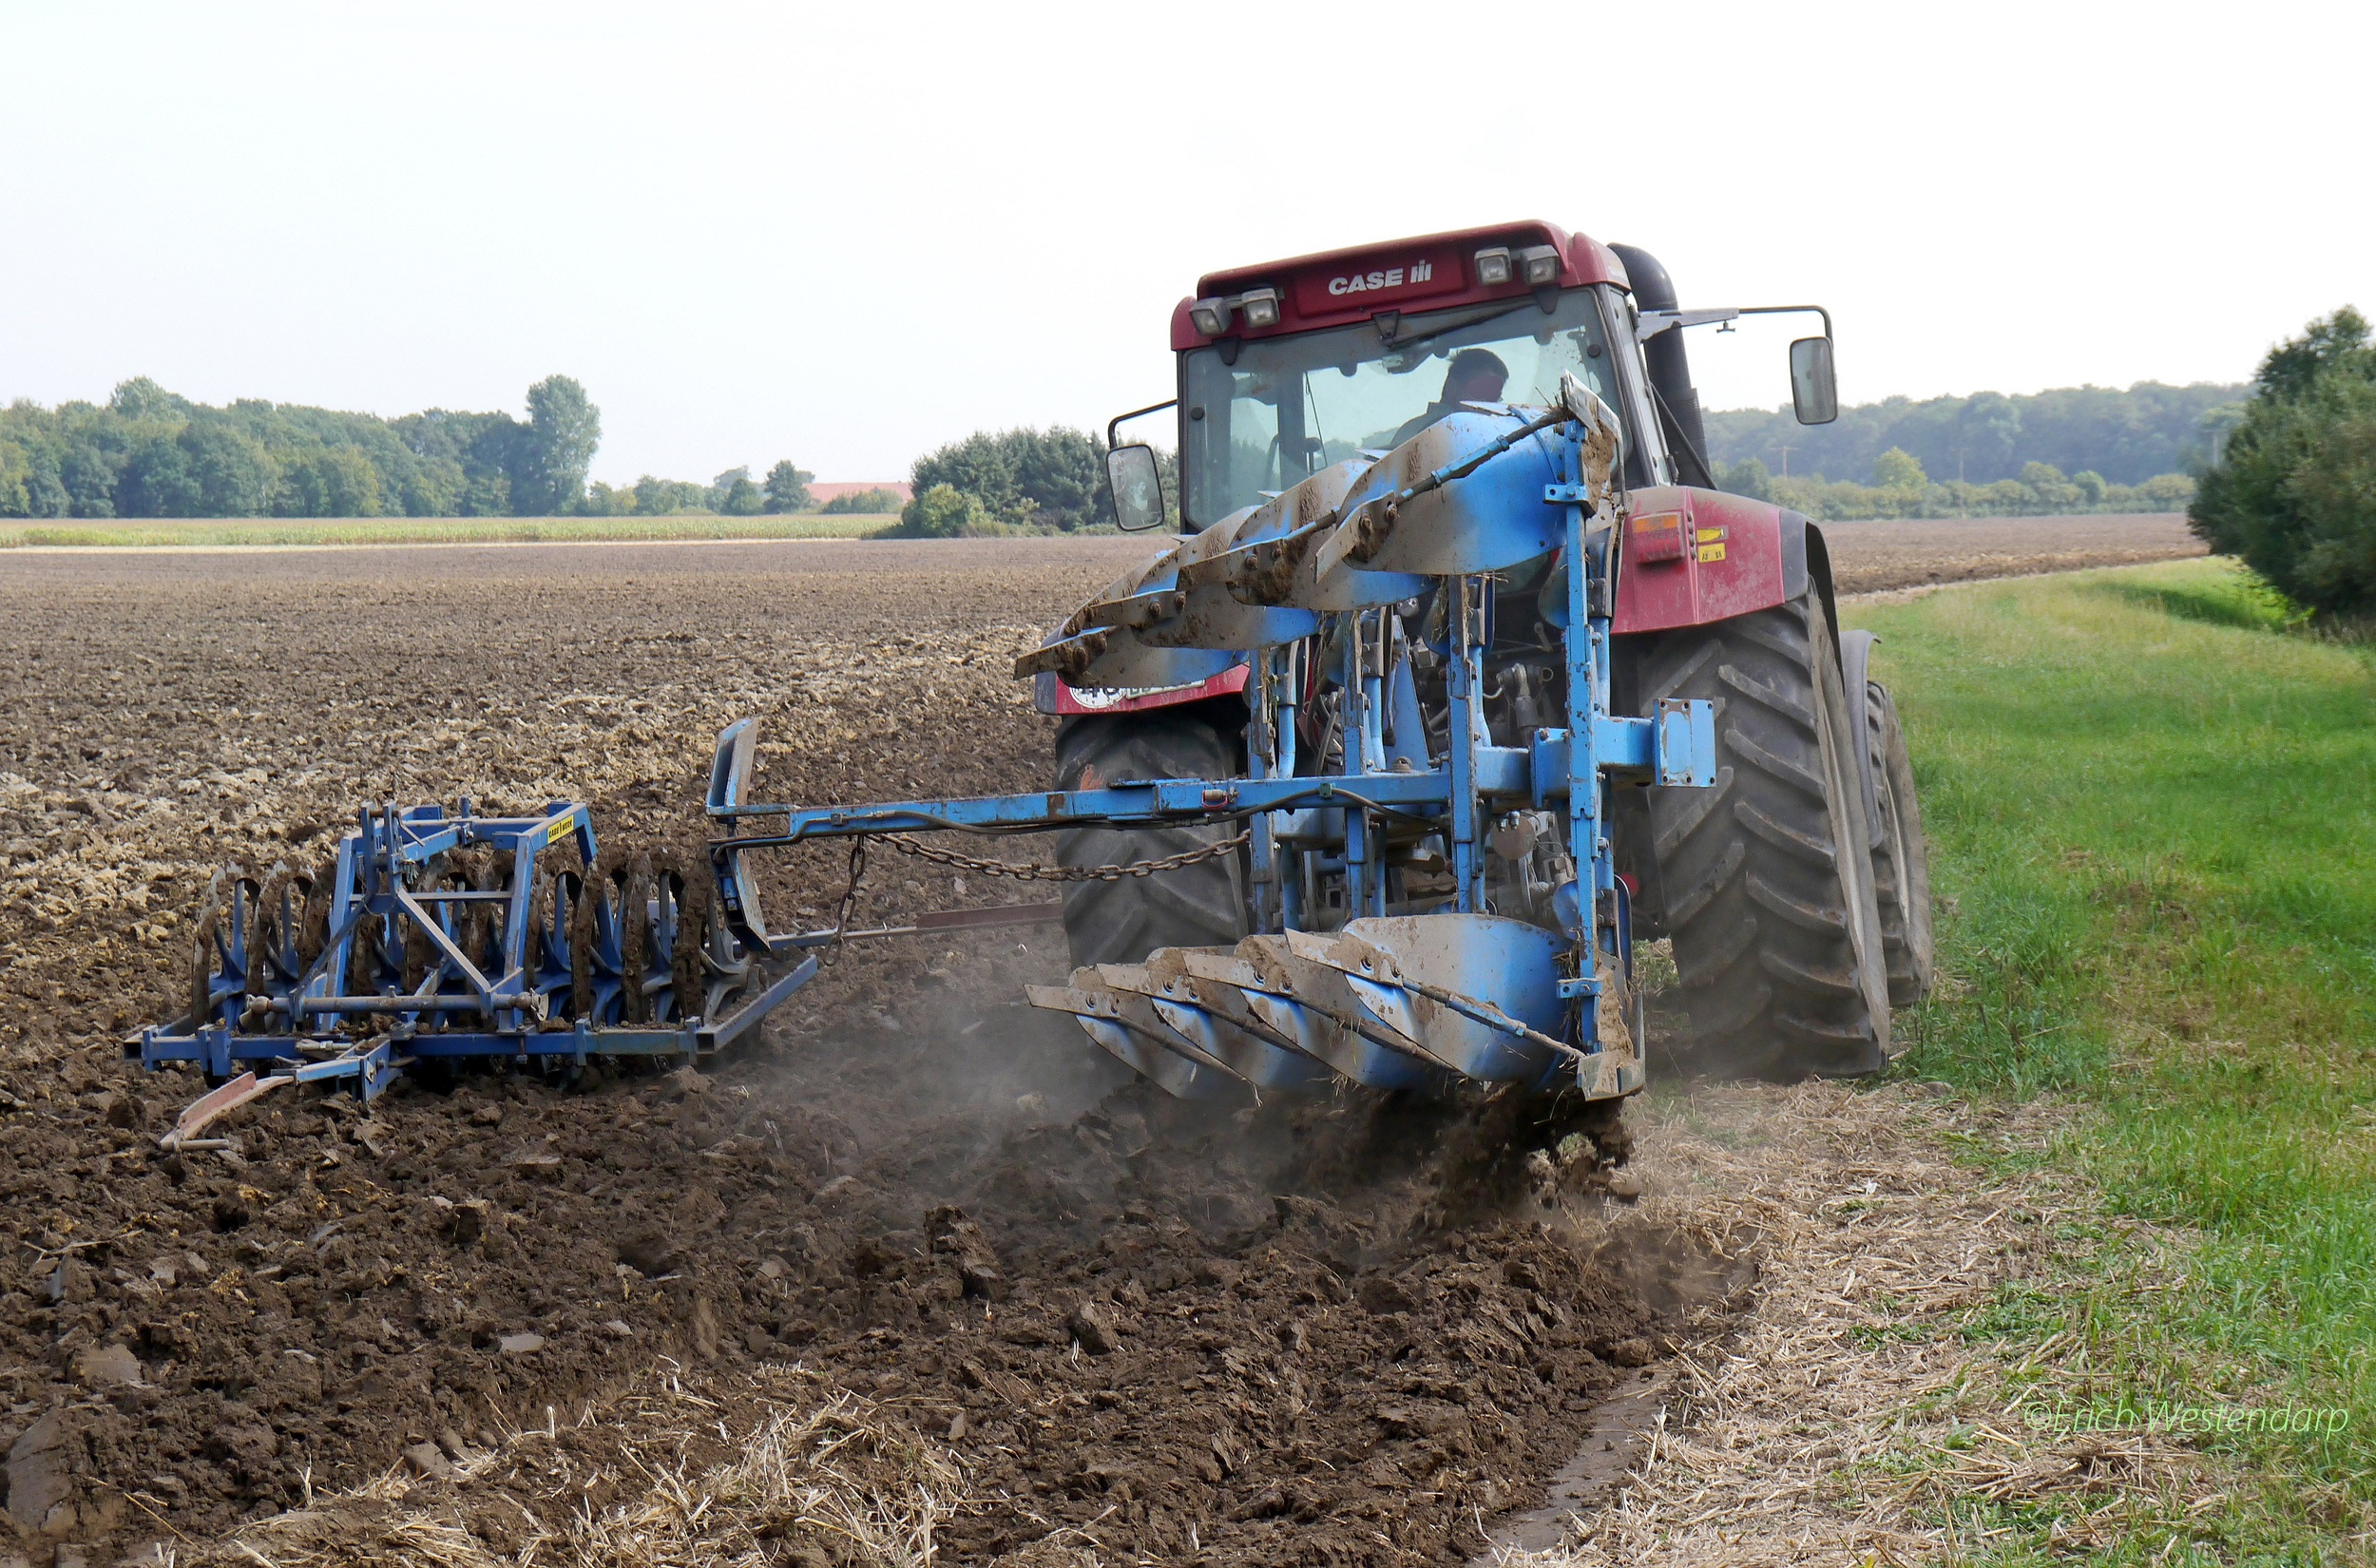
\includegraphics[width=0.8\textwidth]{../foto/lavorazione.jpg}}
  \end{columns}
\end{frame}

\begin{frame}{Parte 2 \small{Azienda agricola Montepaldi (MoLTE)}}
  \begin{overlayarea}{\textwidth}{0.20\textheight}
    \begin{itemize}[<+->]
    \item superficie leggermente declive di circa 15 ha a 90
      m s.l.m.
    \item terreni franco-limosi, calcarei con lenti sabbiose, $pH = 8.3$
    \item area Mediterranea $\rightarrow$ ridotto apporto di concimi
      organici di origine animale
    \end{itemize}
  \end{overlayarea}
  \vfill
  \begin{overlayarea}{\textwidth}{0.45\textheight}
    \only<1>{
      \begin{figure}
        \centering
        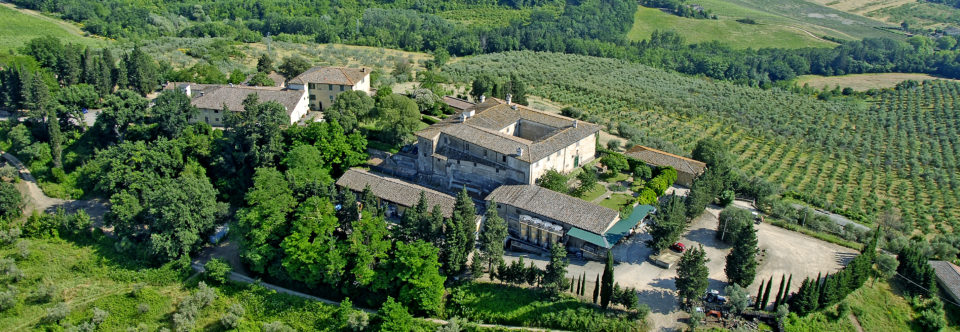
\includegraphics[width=0.9\textwidth]{../foto/Montepaldi.jpg}
      \end{figure}
    }

    \only<2-3>{
      \begin{figure}
        \centering
        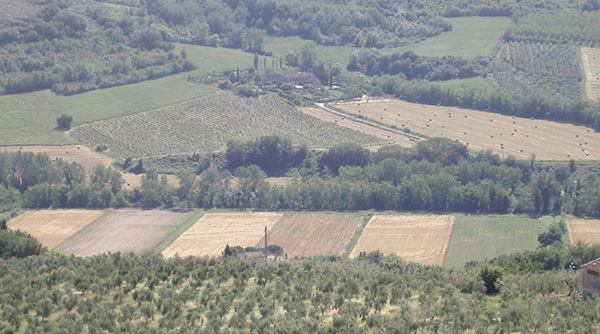
\includegraphics[width=0.7\textwidth]{../foto/campi2.jpg}
      \end{figure}
    }
  \end{overlayarea}  
\end{frame}




\begin{frame}{Parte 2 \small{Aspetti produttivi}}
  % latex table generated in R 3.4.3 by xtable 1.8-2 package
  % Sun Dec 17 09:25:34 2017
  \begin{table}[ht]
    \centering
    \scalebox{0.8}{
      \begin{tabular}{l c p{0.1cm} c c p{0.1cm} c}
        \toprule
        Anno            &           &2016& &          &2017&                \\
                        &&&&&&\\
        Conduzione      & Conv      &    & Bio      & Conv          &&  Bio           \\
        \midrule
                        &&&&&&\\
        Orzo (t/ha)     & 5.00$\pm$ \small{0.05} &&3.40$\pm$
                                                    \small{0.05} &
                                                                   4.30$\pm$ \small{0.06} && 2.50$\pm$ \small{0.06} \\
                        &&&&&&\\
        Girasole (t/ha) & 3.52$\pm$ \small{0.18} &&2.32$\pm$ \small{0.02} &
                                                          \alt<1>{0.25$\pm$ \small{0.07}}{\cellcolor{red!40}{0.25$\pm$ \small{0.07}}} &&
                                                                                                                       \alt<1>{1.18$\pm$ \small{0.09}}{\cellcolor{red!40}{1.18$\pm$ \small{0.09}}}\\
                        &&&&&&\\
        \bottomrule
      \end{tabular}
    }
  \end{table}


\end{frame}



\begin{frame}{Parte 2 \small{Disegno sperimentale}}
  \begin{overlayarea}{\textwidth}{0.20\textheight}  
    \begin{itemize}[<+->]
    \item 4 appezzamenti, 2 Convenzionali e 2 Biologici
    \item 9 parcelle entro appezzamento $\rightarrow$ lavorazioni con 3 repliche
    \item in ogni parcella $\rightarrow$ tre punti campionati in novembre 2016
    \end{itemize}
  \end{overlayarea}
  \begin{overlayarea}{\textwidth}{0.60\textheight}
    \only<1>{
      
      \centering
      \includegraphics[width=0.5\textwidth]{../foto/campi_sperimentali_tracciati.png}
    }
    \only<2>{
      
      \centering
      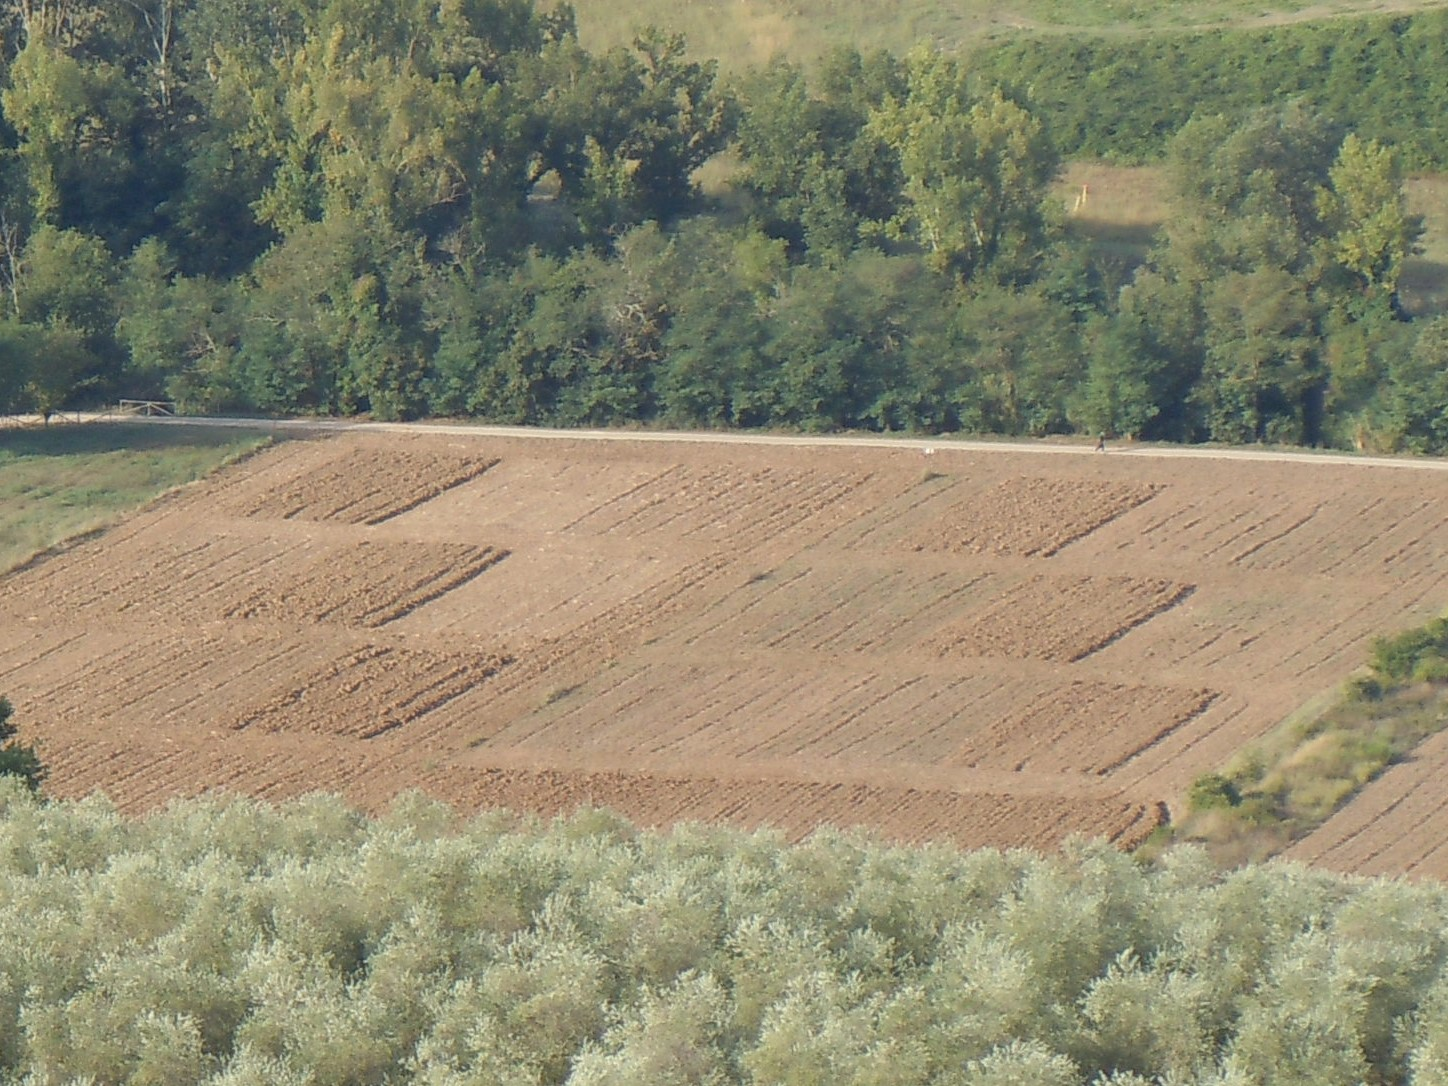
\includegraphics[width=0.65\textwidth]{../foto/Panoramica_lavorazioni.jpeg}
    }
    \only<3-4>{
      \scriptsize
      \begin{table}[ht]
        \centering
        \begin{tabular}{|l|c|c|c|}
          \hline
          &&&\\ 
          Campi        & Convenzionale & Biologico    &\\
          &&&\\
          \hline
          &&&\\ 
          Appezzamenti & 2              &  2          &\\ 
          &&&\\
          \hline
          &&&\\
          Parcelle     &                &             &\\
          entro appezzamento   &      9 &     9       &\\
          &&&\\
          \hline
          &&&\\
          Punti entro  &          3     &    3        &\\ 
          parcella     &&&\\
          \hline
          &&                             &\alt<3>{}{\cellcolor{red!40}{}}   \\
          Totale campioni& 54           &     54      &\alt<3>{108}{\cellcolor{red!40}{108}}   \\
          &&                             &\alt<3>{}{\cellcolor{red!40}{}}   \\
          \hline
        \end{tabular}
      \end{table}
      % 
      % \centering
      % 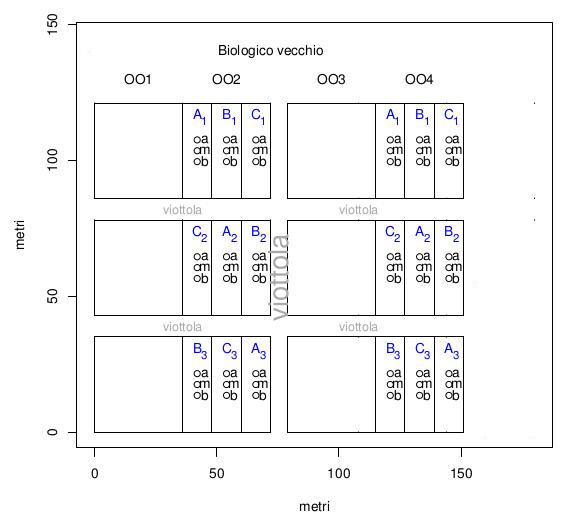
\includegraphics[width=0.5\textwidth]{../foto/OO_sito.jpeg}
      % 
    }%% fine 3-4
  \end{overlayarea}
\end{frame}


\begin{frame}{Parte 2 \small{Metodi di analisi}}
  \begin{columns}[T]
    \column{.50\textwidth}
    \begin{enumerate}
    \item<1->Densità  apparente
      \begin{itemize}
      \item<2-> con cilindro ($854.1\: cm^3$)
      \item<4-> per spinta idrostatica ($\sim 30 \: cm^3$)
      \end{itemize}
    \item<6-> Stabilità degli aggregati
      \begin{itemize}
      \item<7-> secchi all'aria
      \item<7-> pre inumiditi \\  per nebulizzazione
      \end{itemize}
    \item<8-> Porosimetria ad intrusione di mercurio \\ (liquido non bagnante)      
    \end{enumerate}
    \column{.48\textwidth}
    %%%%%%%%%%%%%%% COLONNA SINISTRA dentro overlay area %%%%%%%%%%%%%%%%%%%%%%%%
    \begin{overlayarea}{\textwidth}{0.7\textheight}
      \only<2>{
\centering
        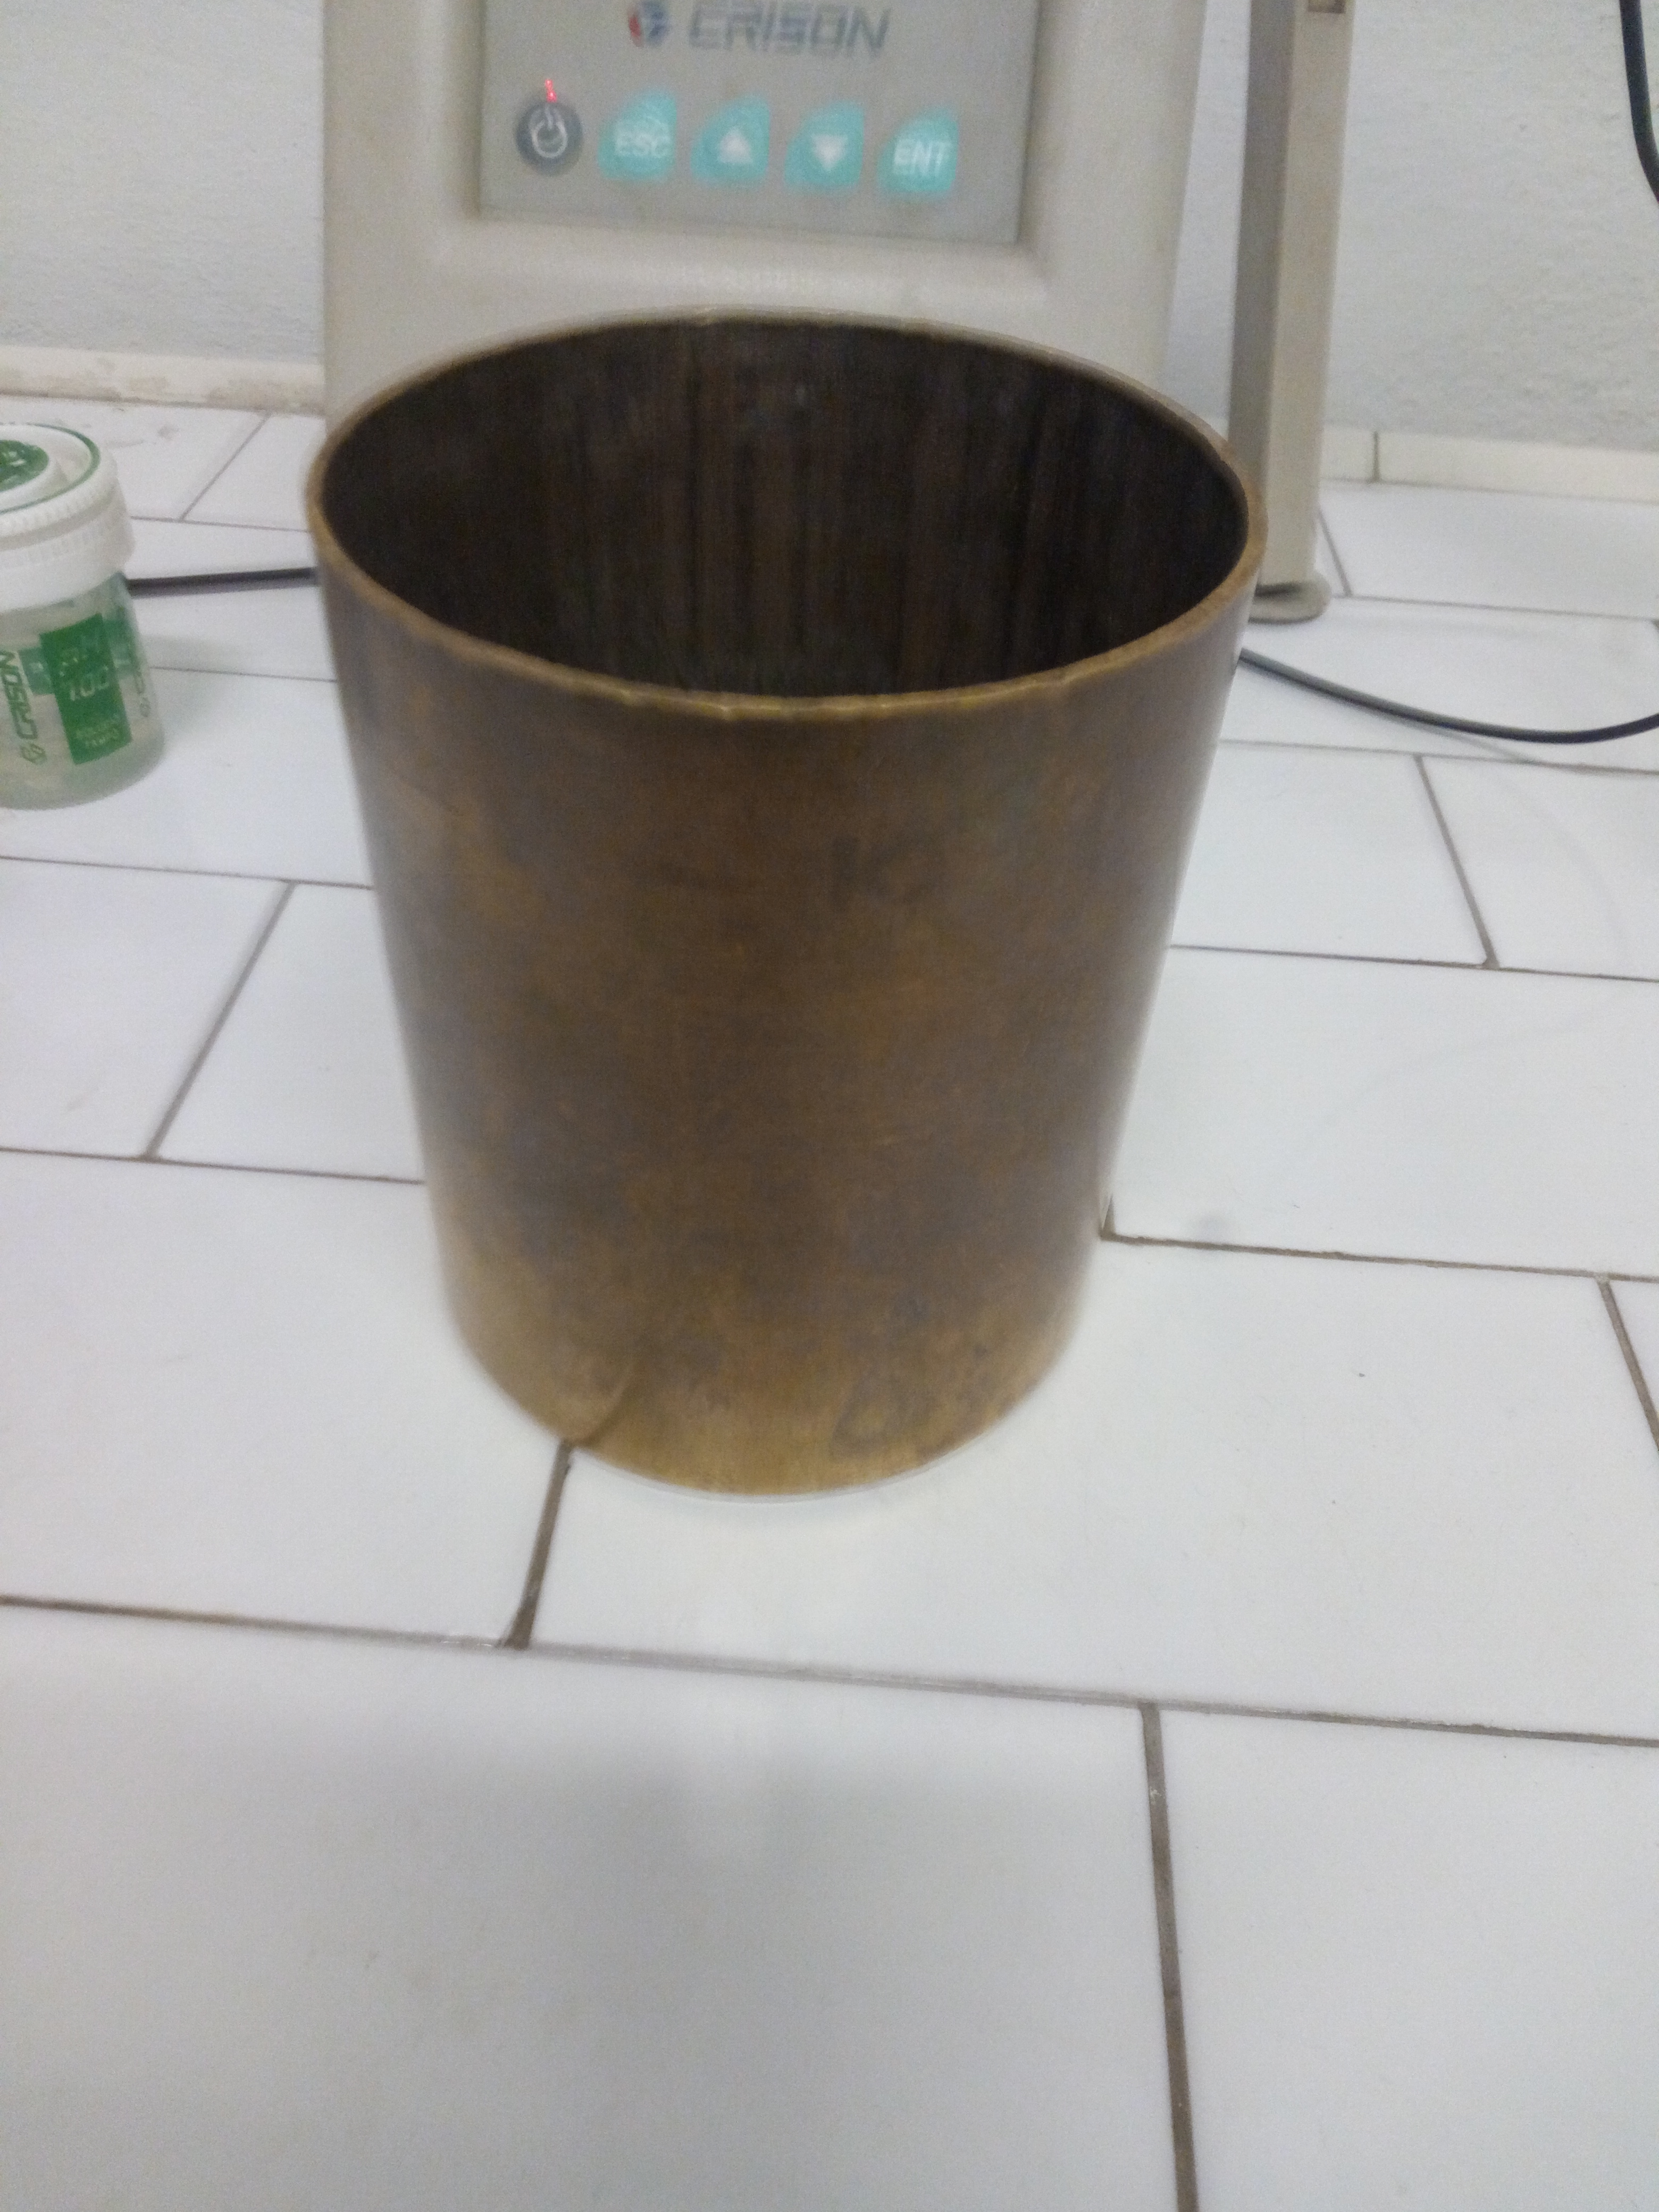
\includegraphics[width=0.8\textwidth]{../foto/cilindroOttone.jpeg}
      }%% fine 2
      \only<3>{
        \vspace{1cm}
\centering
        \[
        D_{App}=\frac{P_{secco}}{V_{cilindro}}
        \]
        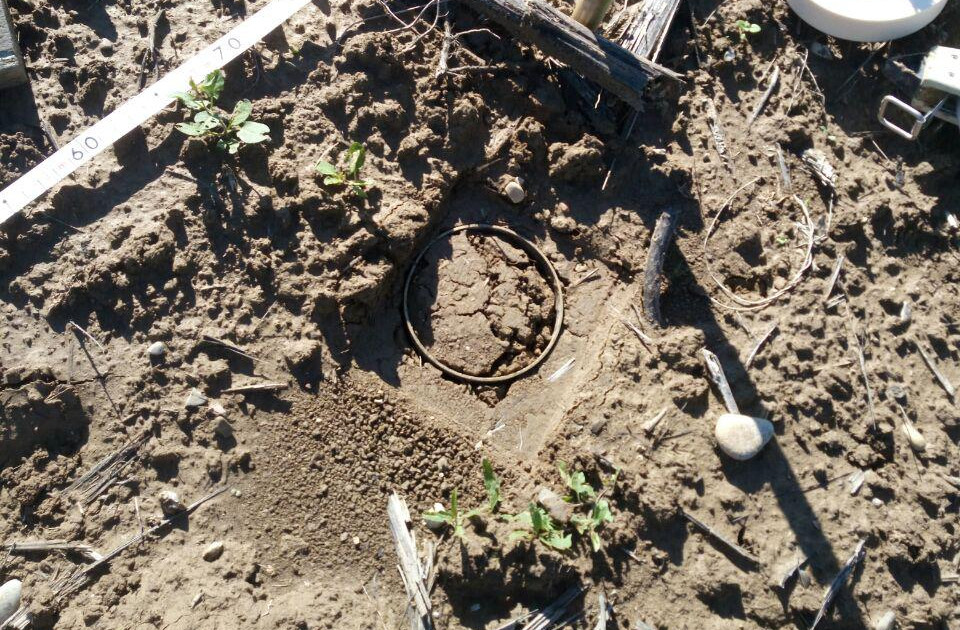
\includegraphics[width=0.8\textwidth]{../foto/cilindrosuolo.jpg}
        
      }%% fine 3
      \only<4>{
\centering
        \vspace{1cm}
        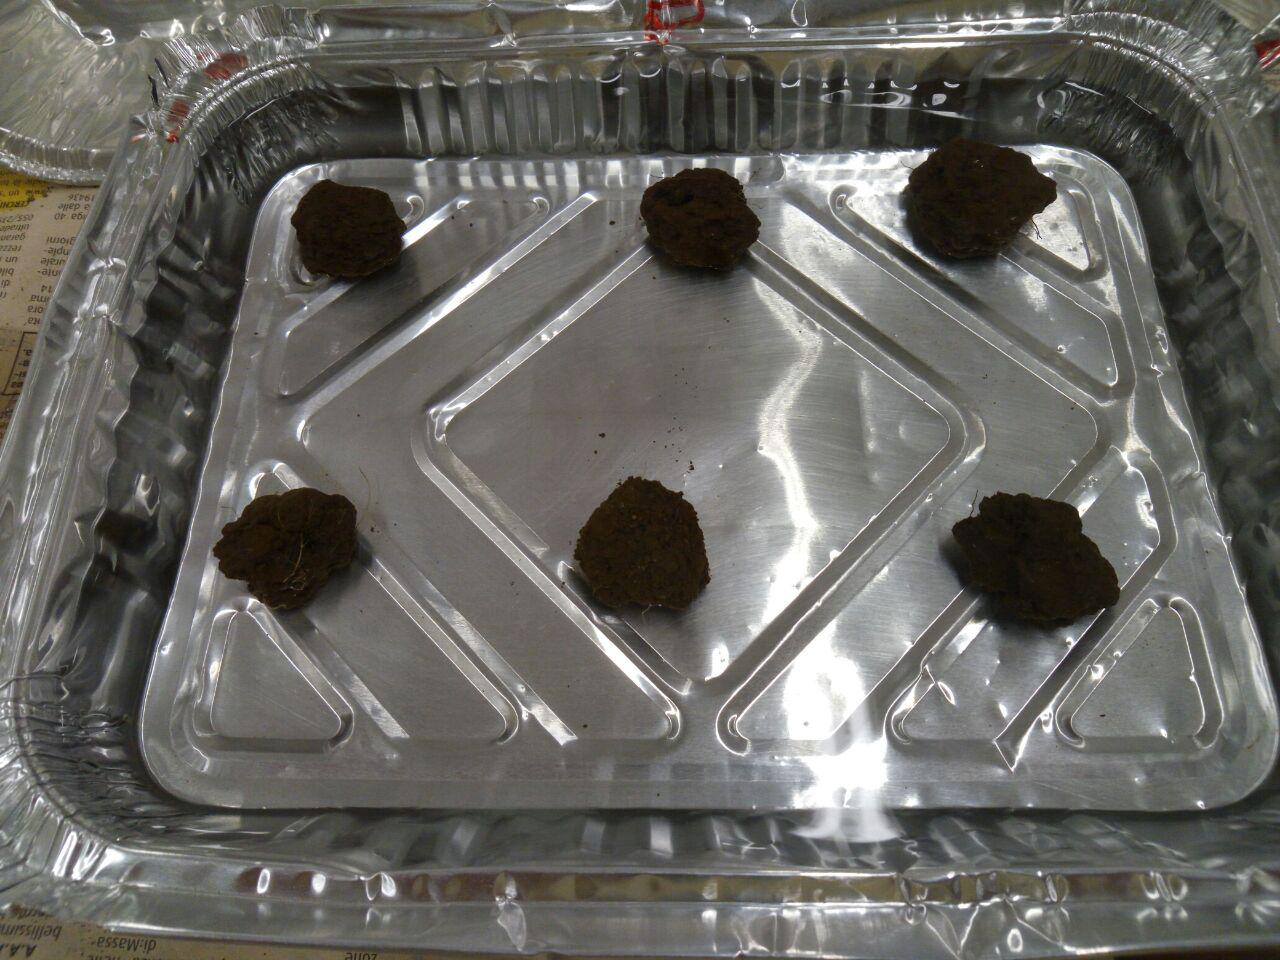
\includegraphics[width=0.8\textwidth]{../foto/petrolio}
        
      }%% fine 4

      \only<5>{
        \centering
        \[
        D_{app} = \frac{P_{aggregato}}{V_{aggregato}}
        \]
        
        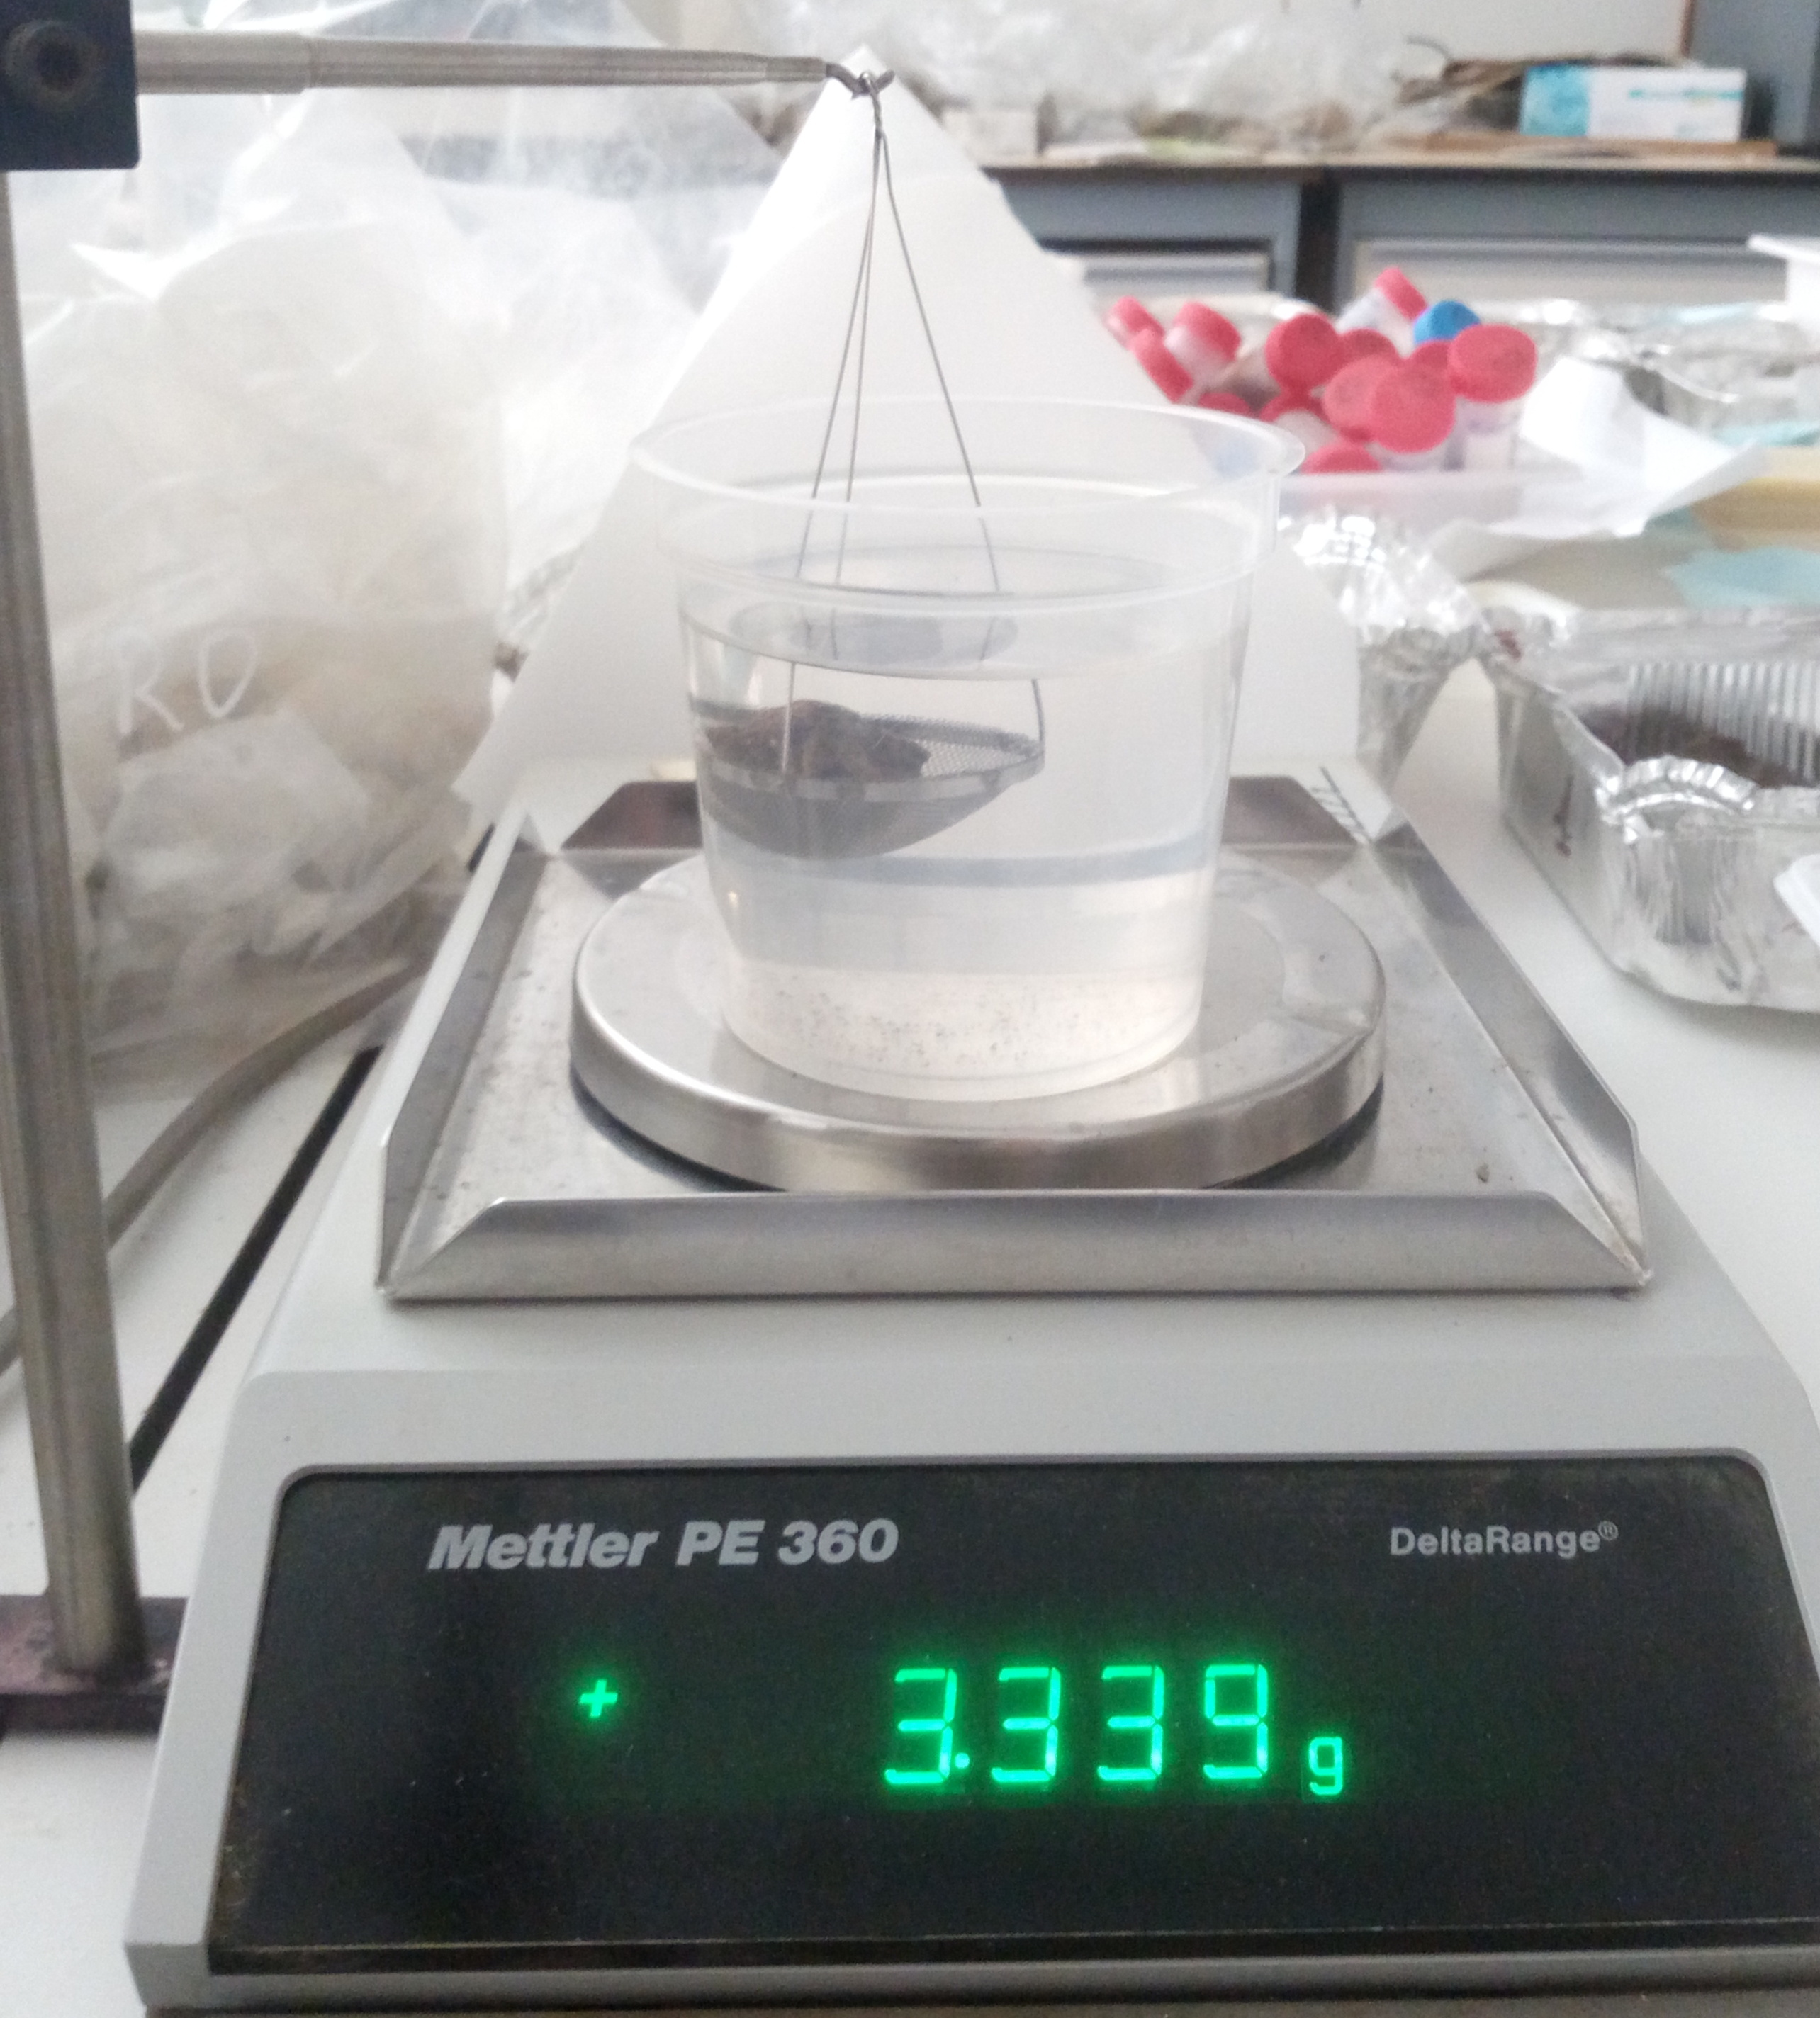
\includegraphics[width=0.8\textwidth]{../foto/spintapeso}
      }%% fine 5

      \only<6>{\animategraphics[loop,autoplay,width=\linewidth]{12}{../foto/stabilitVid/stabilitVid-}{0}{196}
      }%%196 %% fine 6

      \only<7>{\animategraphics[loop,autoplay,width=\linewidth]{12}{../foto/msizer/Msizer-}{117}{176}
        \animategraphics[loop,autoplay,width=\linewidth]{12}{../foto/msizer/Msizer-}{208}{233}
      }%117-176....208-233
       %% fine 7

      \only<8->{
        \centering
        \vspace{1cm}
        \begin{center}
          \animategraphics[loop,autoplay,width=\linewidth]{20}{../foto/poresize/PoreSize-}{0}{396}
        \end{center}

      }%%396 %% fine 8
    \end{overlayarea}   
  \end{columns}
\end{frame}



\begin{frame}{Parte 2 \small{Elaborazione dei dati}}
  %% \transwipe<4>[direction=90]
  \begin{minipage}[0.2\textheight]{\textwidth}
    \begin{columns}[T]
      \column{0.8\textwidth}
      L'elaborazione dei dati è stata effettuata mediante il linguaggio di
      programmazione R, ed ha riguardato:
      \begin{itemize}
        \onslide<2->\item l'adattamento di un modello lineare nella forma:
        \vspace{0.25cm}
        $Y \sim \beta_0 + \beta_1x_1 + \beta_2x_2 + \epsilon$

        \onslide<3->{dove:
          \begin{itemize}
          \item $x_1$ conduzione %\newline
            \emph{Convenzionale}, \emph{Biologico}

          \item $x_2$ lavorazioni \newline \emph{Arato, Rippato,
              Frangizollato}
          \end{itemize}
          Interazioni conduzione*lavorazione non
          significative $\rightarrow$ non considerate nel modello}
      \end{itemize}
      \column{0.2\textwidth}
      \includegraphics[width=2.5cm]{../foto/logo-R.png}
    \end{columns}
  \end{minipage}

  \begin{itemize}
    \onslide<4->\item la validazione del modello attraverso l'analisi
    dei residui 
    \onslide<5->\item verifica della significatività delle
    ipotesi mediante analisi della varianza (ANOVA)
  \end{itemize}
\end{frame}


% \begin{frame}[label=Composizionale]
%   \vspace{2cm}
%   Risultati analisi \hyperlink{Anova}{\beamerbutton{composizionale}}
%   [hb]
%   \includegraphics[width=0.6\textwidth]{../tesi/Tesi_GIT-plotacompWETDRY.pdf}
%   
% \end{frame}

\begin{frame}
  \finalpage{\Huge{Risultati}}
\end{frame}


\begin{frame}[label=Core]{Parte 3 \small{Densità apparente per \bf{\large{cilindro}}}}
  \hyperlink{finale}{\beamerbutton{Conclusioni}}  
  \centering
  \includegraphics[width=0.6\textwidth]{../tesi/boxCore.pdf}
  
\end{frame}

\begin{frame}{Parte 3 \small{Densità apparente con  \bf{\large{cilindro}}}}
  % latex table generated in R 3.4.0 by xtable 1.8-2 package
  % Thu Jun 22 16:16:27 2017

  Tabella ANOVA

  \begin{table}[ht]
    \centering
    \label{tab:anova del modello}
    \begin{tabular}{lrrrrr}
      \toprule
      & Df & SS & MS & F  & Pr($>$F) \\ 
      \midrule 
      Anno         & 1  &  0.02  &  0.02  &   1.41   & 0.2390   \\ 
      Conduzione   & 1  &  0.04  &  0.04  &   3.29   & 0.0745   \\ 
      Lavorazione  & 2  &  0.00  &  0.00  &   0.03   & 0.9728   \\ 
      Residui      & 90 &  0.97  &  0.01  &          &          \\ 
      \bottomrule
    \end{tabular}
  \end{table}
\end{frame}

\begin{frame}[label=Clod]{Parte 3 \small{Densità apparente per \bf{\large{spinta idrostatica}}}}
  \hyperlink{finale}{\beamerbutton{Conclusioni}}
  \only<1>{\centering
    \includegraphics[width=0.6\textwidth]{../tesi/boxCore_SCALA.pdf}
  } 
  \only<2>{
    \centering
    \includegraphics[width=0.6\textwidth]{../tesi/boxClod_SCALA.pdf}
  }
\end{frame}

\begin{frame}{Parte 3 \small{Densità apparente per \bf{\large{spinta idrostatica}}}}
  % latex table generated in R 3.4.0 by xtable 1.8-2 package
  % Thu Jun 22 16:32:35 2017
  % Thu Jun 22 16:16:27 2017

  Tabella ANOVA

  
  \begin{table}
    \centering
    \begin{tabular}{llcccc}
      \toprule
      & Df  & SS & MS & F & Pr($>$F) \\ 
      \midrule
      Conduzione  & 1   & 0.03   & 0.03    & 6.31    & 0.012    \\ 
      Lavorazione & 2   & 0.05   & 0.02    & 5.83    & 0.004    \\ 
      Totale      & 104 & 0.42   & 0.00    &         &          \\ 
      \bottomrule
    \end{tabular}
    \label{tab:Anova densita per spinta}
  \end{table}

\end{frame}

\begin{frame}{Parte 3 \small{Densità apparente con \bf{\large{spinta idrostatica}}}}

  \footnotesize
  \begin{table}[ht]
    \centering
    \begin{tabular}{llrccc}
      \toprule
      \\
      Conduzione    & Lavorazione   & Media& Dev. std & n    & Tukey \\ 
      \\
      \midrule
      \\
      Convenzionale & Arato         & 1.93 & 0.06      &  18 & b     \\ 
                    & Frangizollato & 1.89 & 0.05      &  18 & ab    \\ 
                    & Rippato       & 1.90 & 0.06      &  18 & ab    \\
      \\
      Biologico     & Arato         & 1.90 & 0.07      &  18 & ab    \\ 
                    & Frangizollato & 1.84 & 0.06      &  18 & a     \\ 
                    & Rippato       & 1.87 & 0.07      &  18 & ab    \\ 
      \\
      \bottomrule
    \end{tabular}
    \label{tab:RiassuntoDensitaSpinta}
  \end{table}
\end{frame}


\begin{frame}{Parte 3 \small{Stabilità degli aggregati}}
\begin{center}
\LARGE Stabilità degli aggregati

\vspace{1.5cm}

    \includegraphics[width=0.45\textwidth]{../foto/msizer/Msizer-78}
    \includegraphics[width=0.45\textwidth]{../foto/msizer/Msizer-218}
\end{center}
\end{frame}


\begin{frame}{Parte 3 \small{Stabilità degli aggregati}}
  %\transdissolve<2>
  %   %% \begin{columns}
  %   %%   \column{.50\textwidth}
  %   %%   \vspace{1cm}
  %   %%   \footnotesize
  %   %%   \begin{itemize}[<+->]
  %   %%   \item 
  %     \begin{center}
  %       Dati ottenuti dalle analisi di porosimetria e\\
  %       stabilità degli aggregati $\rightarrow$ \emph{dati
  %       Composizionali}%sono delle distribuzioni in cui ogni
  %     \end{center}

  %     \vfill
  %   %   %     classe dimensionale è espressa come percentuale sul volume totale,
  %   %   %     questo tipo di dati prende il nome di
  %   %     \pause
  %   %   \item Per rappresentare i dati composizionali si utilizza un
  %   %     grafico triangolare. Per l'elaborazione è necessaria
  %   %     un'operazione di linearizzazione
  %   %   \item Operazioni sono state effettuate tramite il package 'composition'
  %   %   \end{itemize}
  %   \vfill
  %   %%   \column{.48\textwidth}
  \only<1>{%%\begin{overlayarea}{\linewidth}{3cm}
    
    \centering
    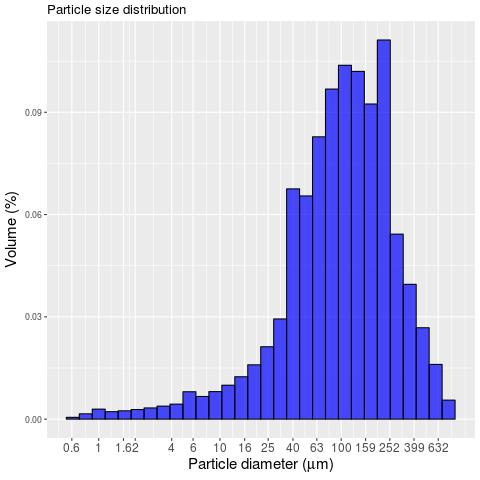
\includegraphics[width=0.5\textwidth]{../grafici/HistoStab.jpeg}
    
  }
  \only<2>{%%\begin{overlayarea}{\linewidth}{3cm}
    
    \centering
    \includegraphics[width=0.8\textwidth, page=1]{../grafici/SplitStabHoBarato.pdf}
    
  }
  %% \end{overlayarea}}
  %   %% \only<3>{\includegraphics[width=0.5\textwidth]{../foto/simplessodeformaVerticale.png}}
  \only<3>{
    
    \centering
    \includegraphics[width=0.75\textwidth, page=1]{../grafici/stabilita.pdf}
    
  }  %% \end{columns}
  \only<4>{
    \begin{center}
      \animategraphics[autoplay,width=0.75\linewidth]{6}{../grafici/stabilita}{1}{11}
    \end{center}
  }
  \only<5>{
    \begin{center}
      \animategraphics[autoplay,width=0.75\linewidth]{6}{../grafici/stabilita}{11}{22}
    \end{center}
  }

\end{frame}





\begin{frame}[label=distribuzione]{Parte 3 \small{Stabilità degli aggregati}}
  % \hyperlink{finale}{\beamerbutton{Conclusioni}} 
  %\transdissolve<1-2, 5-6>[duration=0.8]
  \only<1>{
    \centering
    \includegraphics[width=0.75\textwidth, page=25]{../grafici/stabilita.pdf}

  }
  \only<2>{
    \centering
    \includegraphics[width=0.75\textwidth, page=26]{../grafici/stabilita.pdf}

  }
  \only<3>{
    \centering
    \includegraphics[width=0.75\textwidth, page=27]{../grafici/stabilita.pdf}

  }
  \only<4>{
    \centering
    \includegraphics[width=0.75\textwidth, page=28]{../grafici/stabilita.pdf}

  }
  \only<5>{
    \centering
    \includegraphics[width=0.75\textwidth, page=32]{../grafici/stabilita.pdf}

  }
  \only<6>{
    \centering
    \includegraphics[width=0.75\textwidth, page=33]{../grafici/stabilita.pdf}

  }
\end{frame}



\begin{frame}[label=Anova]{Parte 3 \small{Stabilità degli aggregati}}
  \hyperlink{Composizionale}{\beamerbutton{Conclusioni}}
  \footnotesize
  % latex table generated in R 3.4.0 by xtable 1.8-2 package
  % Tue Jun 27 21:29:19 2017
  Tabella ANOVA 
  \begin{table}
    \centering
    \begin{tabular}{lrrrrcr}
      \toprule
      & Df&Pillai& approx F & num Df & den Df & Pr($>$F) \\ 
      \midrule
      Convenzionale & 1 & 0.92 & 4955.26  &      2 &    835 & $<10^{-3}$\\ 
      Biologico     & 1 & 0.09 & 41.72    &      2 &    835 & $<10^{-3}$\\ 
      Tempo         & 1 & 0.92 & 4504.77  &      2 &    835 & $<10^{-3}$\\ 
      Tempo$^2$     & 1 & 0.35 & 227.06   &      2 &    835 & $<10^{-3}$\\ 
      Totale        & 836 &    &          &        &        &          \\ 
      \bottomrule
    \end{tabular}
  \end{table}
\end{frame}

\begin{frame}{Parte 3 \small{Distribuzione dimensionale dei pori}}
\begin{center}
\LARGE Distribuzione delle dimensioni dei pori

\vspace{1.5cm}

    \includegraphics[width=0.45\textwidth]{../foto/poresize/PoreSize-48.png}
    \includegraphics[width=0.45\textwidth]{../foto/poresize/PoreSize-378.png}
\end{center}
\end{frame}


\begin{frame}[label=Porosimetria]{Parte 3 \small{Distribuzione dimensionale dei pori}}
\begin{columns}
\column{.32\textwidth}
\footnotesize{
Pori classificati in base alle funzioni:
\begin{itemize}
    \item Transmission \\ più grandi, \\acqua in movimento
    \item Storage \\ intermedi,\\ acqua disponibile per le
      piante
    \item Residuals \\ più piccoli,\\acqua non disponibile
      per le piante
\end{itemize}}
\hyperlink{finale}{\beamerbutton{Conclusioni}}
\column{.66\textwidth}
  
  \begin{figure}
    \includegraphics[width=\textwidth]{../grafici/AcompPORO.pdf}
  \end{figure}

\end{columns}
\end{frame}

\begin{frame}{Parte 3 \small{Distribuzione dimensionale dei pori}}

  \footnotesize
  \begin{table}[hb]
    \centering
    % \caption{Distribuzione dei pori nelle tre classi dimensionali
    % dei dati ottenuti dalla analisi
    % con porosimetria a mercurio}
    % \label{tab:Poro_medie}
    \begin{tabular}{llccc}%p{1.25cm}p{3.25cm}p{2cm}}
      
      \toprule
      \\
   &             & Pori    & Pori di         & Pori di\\
      Conduzione & Lavorazione & residuali & immagazzinamento &
                                                                trasmissione \\ 
   &             & (\%) &  (\%) &  (\%) \\
      \\
      \midrule
      \\
      Convenzionale & Arato & 74 & 24 & 2 \\ 
   & Rippato & 61 & 34 & 6 \\ 
   & Frangizollato & 65 & 33 & 2 \\ 
   &  &  &  &  \\ 
      Biologico & Arato & 56 & 41 & 3 \\ 
   & Rippato & 56 & 41 & 3 \\ 
   & Frangizollato & 64 & 32 & 4 \\ 
      \\
      \bottomrule
    \end{tabular}
  \end{table}
\end{frame}

\begin{frame}{Parte 3 \small{Distribuzione dei pori}}
  Tabella ANOVA 
  \begin{table}[ht]
    \centering
    % \caption{Analisi della varianza relativa al modello
    % composizionale dei dati ottenuti dalle analisi con porosimetria
    % a mercurio }
    % \label{tab:poros_anova}
    \begin{tabular}{lrrrrrr}
      \toprule
      & Df & Pillai & approx F & num Df & den Df & Pr($>$F) \\ 
      \midrule
      Intercetta & 1 & 0.94 & 60.45 & 2 & 7 & $<10^{-3}$ \\ 
      Conduzione & 1 & 0.14 & 0.58 & 2 & 7 & 0.585 \\ 
      Lavorazione & 2 & 0.52 & 1.41 & 4 & 16 & 0.275 \\ 
      Totale & 8 &  &  &  &  &  \\ 
      \bottomrule
    \end{tabular}
  \end{table}
\end{frame}




\begin{frame}[label=finale]{Parte 4 \small{Conclusioni I}}
  \begin{enumerate}[<+->]
  \item densità apparente:
    \begin{itemize}
    \item metodo con \hyperlink{Core}{\beamerbutton{CILINDRO}} semplicità esecutiva,
      nessuna differenza significativa
    \item metodo per \hyperlink{Clod}{\beamerbutton{SPINTA}}
      differenze significative, ma di lieve entità.
    \end{itemize}
  \item \hyperlink{distribuzione}{\beamerbutton{STABILITA'}} dinamica:
    aggregati da appezzamenti \emph{convenzionali} più stabili,
    lavorazioni non significative.
  \item \hyperlink{Porosimetria}{\beamerbutton{PORI}}: tendenza  dei suoli
    \emph{biologici} ad avere più pori di immagazzinamento.
  \end{enumerate}

\end{frame}

\begin{frame}{Parte 4 \small{Conclusioni II}}
  I tre parametri misurati indicano che:
  \begin{itemize}[<+->]
    \pause
  \item La conduzione convenzionale esibisce una maggiore stabilità
    alla rottura degli aggregati
  \item La conduzione biologica  per contro possiede una maggiore
    porosità e una tendenza ad ad avere pori più grandi
  \item Gli effetti delle lavorazioni sono di minima entità se non nulle
  \end{itemize}

\end{frame}



\begin{frame}
  \finalpage{\LARGE{Grazie per l'attenzione}}
\end{frame}

%%% Local Variables:
%%% mode: latex
%%% TeX-master: t
%%% End:
%%\appendix



\begin{frame}
  \footnotesize
  \begin{table}[ht]
    \centering
    \caption{Sintesi dei dati della porosit\`a totale ricavati dalle analisi della porosimetria a mercurio} 
    \label{tab:tot_sommario}
    \begin{tabular}{llSScc}%llcccc}
      \toprule
      {Conduzione} & {Lavorazione} & {Porosità totale} & {ST.DEV} & {n} & {Tukey} \\ 
      \midrule
      Convenzionale & Arato & 159.91 & 16.21 &   2 & a \\ 
                   & Rippato & 168.37 & 20.92 &   3 & a \\ 
                   & Frangizollato & 186.13 & 30.38 &   3 & a \\ 
                   &  &  &  &  &  \\ 
      Biologico & Arato & 168.03 & 9.62 &   2 & a \\ 
                   & Rippato & 192.20 & 38.54 &   4 & a \\ 
                   & Frangizollato & 218.28 & 7.29 &   2 & a \\ 
      \bottomrule
    \end{tabular}
  \end{table}
\end{frame}

\begin{frame}
\vskip 1.5cm
\begin{figure}
\centering
\includegraphics[width=0.7\textwidth, page=3]{../grafici/RisultatiChimica-Fisica.pdf}
\end{figure}
\end{frame}

\begin{frame}
  \vskip 1.5cm
  \begin{figure}
    \centering
    \includegraphics[width=0.6\textwidth,
    page=1]{../grafici/PCA_penetrometria_LavorazETConduz.pdf} 
  \end{figure}
\end{frame}


\begin{frame}
  \vskip 1.5cm
  \begin{figure}
    \centering
    \includegraphics[width=0.6\textwidth,
    page=2]{../grafici/PCA_penetrometria_LavorazETConduz.pdf} 
  \end{figure}
\end{frame}


\begin{frame}
  \vskip 1.5cm
  \begin{figure}
    \centering
    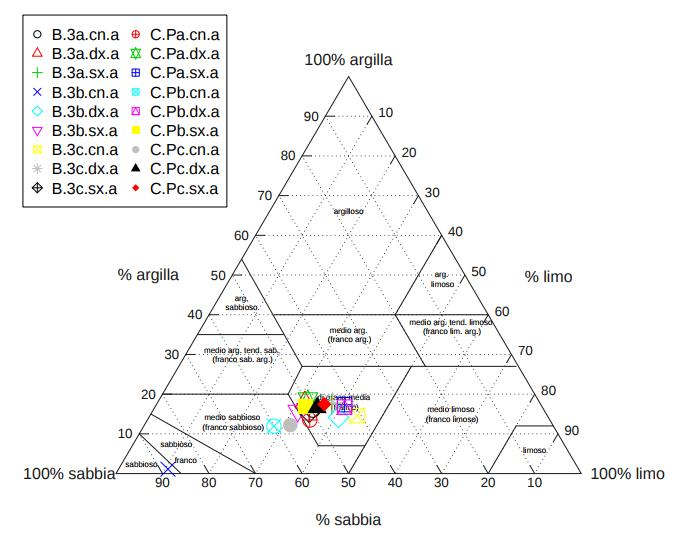
\includegraphics[width=0.6\textwidth]{../foto/USDA_triangolo} 
  \end{figure}
\end{frame}

\begin{frame}
  \vskip 1.5cm
  \begin{figure}
    \centering
    \includegraphics[width=\textwidth]{../foto/simplessodeforma} 
  \end{figure}
\end{frame}





\end{document}

%%% Local Variables:
%%% mode: latex
%%% TeX-master: t
%%% End:
